\documentclass[10pt]{beamer}
\usepackage{ragged2e}
\usepackage{hyperref}
\usepackage{wrapfig}
\usepackage{etoolbox}
\usepackage{multicol}
\apptocmd{\frame}{}{\justifying}{}
\apptocmd{\block}{}{\justifying}{}
\usetheme[]{Aalborg}
  
\setbeamercolor{Aalborg}{fg=purple!20,bg=purple}
%\setbeamercolor{sidebar}{bg=red!20}
% Change the color of the structural elements:
\setbeamercolor{structure}{fg=purple}
% Change the frame title text color:
%\setbeamercolor{frametitle}{fg=blue}
% Change the normal text color background:
%\setbeamercolor{normal text}{bg=gray!10}

\usepackage[utf8]{inputenc}
\usepackage[english]{babel}
\usepackage[T1]{fontenc}
\usepackage{helvet}


% colored hyperlinks
\newcommand{\chref}[2]{%
  \href{#1}{{\usebeamercolor[fg]{Aalborg}#2}}%
}

\title[Where are they looking]% optional, use only with long paper titles
{Where are they looking?}

\subtitle{Topicos de Investigación I}  % could also be a conference name

%\date{\today}
\date{\vspace{-3.5ex}}

\author[Team Bomb!] % optional, use only with lots of authors
{
  Arotoma Bacilio, Bitzer Nazareth\\
  Bedon Vasquez, Bruno Fabio\\
  Huarcaya Canal, Oscar\\
  Mejia Puma, Miguel Angel\\  
%  \href{mailto:ohuarcaya.c@gmail.com}{{\tt ohuarcaya.c@gmail.com}}
}
% - Give the names in the same order as they appear in the paper.
% - Use the \inst{?} command only if the authors have different
%   affiliation. See the beamer manual for an example

\institute[
%  {\includegraphics[scale=0.2]{aau_segl}}\\ %insert a company, department or university logo
  FC - UNI\\
  Computer Science
] % optional - is placed in the bottom of the sidebar on every slide
{% is placed on the bottom of the title page
  Universidad Nacional de Ingeniería\\
  Facultad de Ciencias\\
  Escuela Profesional de Ciencia de la Computación  
  %there must be an empty line above this line - otherwise some unwanted space is added between the university and the country (I do not know why;( )
}

% specify the logo in the top right/left of the slide
\pgfdeclareimage[height=1cm]{mainlogo}{AAUgraphics/log_uni} % placed in the upper left/right corner
\logo{\pgfuseimage{mainlogo}}

% specify a logo on the titlepage (you can specify additional logos an include them in 
% institute command below
\pgfdeclareimage[height=2.5cm]{titlepagelogo}{AAUgraphics/log_uni} % placed on the title page
%\pgfdeclareimage[height=1.5cm]{titlepagelogo2}{AAUgraphics/aau_logo_new} % placed on the title page
\titlegraphic{% is placed on the bottom of the title page
  \pgfuseimage{titlepagelogo}
%  \hspace{1cm}\pgfuseimage{titlepagelogo2}
}

\begin{document}
% the titlepage
{\aauwavesbg
\begin{frame}[plain,noframenumbering] % the plain option removes the sidebar and header from the title page
  \titlepage
\end{frame}}
%%%%%%%%%%%%%%%%

% TOC
%\begin{frame}{Contenido}{}
%\tableofcontents
%\end{frame}
%%%%%%%%%%%%%%%%
%
% Diapositivas .................................................
%
%%%%%%%%%%%%%%%%
\section{Introducción}
\begin{frame}{Introducción}{}
\begin{block}{Detalles del Trabajo}
%La temática del presente estudio consiste en evaluar %el comportamiento
%como se desempeñan
%de 
%los modelos de aprendizaje supervisado que Machine Learning ofrece.

%Con ese fin se usan los datos de localización de interiores por sensores
%bluetooth 4.0, basados en intensidad de señal RSSI.\\
\begin{wrapfigure}{l}{0.3\textwidth}
    \centering
    \includegraphics[width=0.3\textwidth]{AAUgraphics/neural-icon}
  \end{wrapfigure}
\ \\El desarrollo del presente trabajo\\incluye:
	\begin{itemize}
    \item[1.] Estructuración de los datos.
    \item[2.] Preparación de los modelos.
    \item[3.] Evaluación de modelos.%por emisor, receptor e intensidad.
    \item[4.] Validación de resultados.
    \item[5.] Análisis y Conclusiones.
  \end{itemize}
  
\end{block}
\end{frame}

\subsection{Porqué localización de interiores}
\begin{frame}{Introducción}{Porqué localización de interiores}
%Hoy en día, existe un gran interés en el desarrollo e implementación de 
%servicios orientados a la localización en interiores.
Las aplicaciones más frecuentes son:
\begin{itemize}
	\item[•] Marketing en retail \textit{(publicidad, oferta, cupones)}.
	\item[•] Orientación en interiores \textit{(guías)}.
	\item[•] Eficiencia en la atención \textit{(grado de incidencia)}.
\end{itemize}
\includegraphics[width=10cm,height=4cm]{AAUgraphics/indoor}
%https://juassic.com/files/images/posts/bigstock-City-Map-With-Pins-And-An-Inte-96261419.jpg
\end{frame}

\subsection{Porqué Machine Learning}
\begin{frame}{Introducción}{Porqué Machine Learning}
\begin{block}{Soluciones para indoor location}
%\begin{justify}
%Para localización de interiores con RSSI de Beacons bluetooth, se puede utilizar 
%una función de distancia: 
\begin{center}
\includegraphics[scale=0.3]{AAUgraphics/ips}
\end{center}
Ecuación de Rappaport:
$$RSSI = -10 n log(d) + txPower$$
%Donde $d$ = distance, $n$ = cte. de propagación de señales$^{\href{www.mydick.exls}{[1]}}$.
%Pero n = 2 en un espacio libre, pero variará según la geometría local. 
%Por ejemplo una pared reduce RSSI en $\sim 3dBm$. Además tiene un error promedio de $5m$, 
%dependiendo de las condiciones.\\
Propuesta:\\
\begin{center}
Modelar usando Machine Learning.
\end{center}
%Una propuesta es el uso de modelos de aprendizaje supervisado de Machine Learning, si el 
%error promedio (en distancia) es menor a $5m$; entonces esta propuesta ofrece mejor calidad de 
%resultados. Además tenemos una amplia variedad de algoritmos que obtendrán diferentes resultados.
%\end{justify}
\end{block}
\end{frame}

\subsection{Definición del Problema}
\begin{frame}{Introducción}{Definición del Problema}
\begin{block}{Area Experimental}
%\begin{multicols}{2}
%\begin{justify}
%El interior experimental mide $9.3m$ de largo y $6.3m$ de ancho, en donde se 
%distribuyen quince sectores de $1m^2$ con separación de $0.5m$ vertical y horizontal.
%Además, se dejo una franja de $1.15m$ al borde del interior.
%\end{justify}
\begin{center}
\includegraphics[scale=0.6]{AAUgraphics/sensors}
\end{center}
%\end{multicols}
%\begin{justify}
%Los cinco puntos de la imágen son emisores bluetooth (Beacon BLE 4.0 y Microcontroller), el receptor (Smartphone y Raspberry Pi con antena usb BLE 4.0) se coloca en cada uno de los quince sectores y se extraen las medidas RSSI de cada emisor.
%\end{justify}
\end{block}
\end{frame}

\section{Indoor Location}
\begin{frame}{Indoor Location}{}
\begin{block}{Casos de Prueba}
El presente trabajo evalua la eficiencia para tres tipos de sucesos.\\
\begin{itemize}
	\item Caso 1:\\
	\textbf{Emisor:} Microcontroller BLE 4.0, a un único nivel de potencia.\\
	\textbf{Receptor:} Raspberry Pi con antena BLE 4.0.
	
	\item Caso 2:\\
	\textbf{Emisor:} Beacon BLE 4.0, a siete niveles de potencia.\\
	\textbf{Receptor:} Raspberry Pi con antena BLE 4.0.
	
	\item Caso 3:\\
	\textbf{Emisor:} Beacon BLE 4.0, a siete niveles de potencia.\\
	\textbf{Receptor:} Smartphone BLE 4.0.
\end{itemize}
\end{block}
\end{frame}

\subsection{Casos de Prueba}
\begin{frame}{Indoor Location}{Casos de Prueba}
\begin{block}{Caso 1: microController $\rightarrow$ RPI2}
%Por el coeficiente de correlación de Pearson en el siguiente gráfico se tiene que no hay relación lineal para Be07, Be08, Be09, Be10 y algo muy ligero para Be11.\\
\begin{multicols}{2}
\includegraphics[scale=0.3]{AAUgraphics/correlationCon.eps}
%\\El Sector tiene una relación lineal inversa débil con Be09 y lineal débil con Be10.
\end{multicols}
\end{block}
\end{frame}

\begin{frame}{Indoor Location}{Casos de Prueba}
\begin{block}{Caso 2: Beacon $\rightarrow$ RPI2}
%Se tiene las coeficientes de correlación para los siete niveles de potencia de los beacons sobre Raspberry. En ciertos casos se observa cierta relación lineal (Be11 y Sector en Tx=0x01,0x02,0x06)
\begin{center}
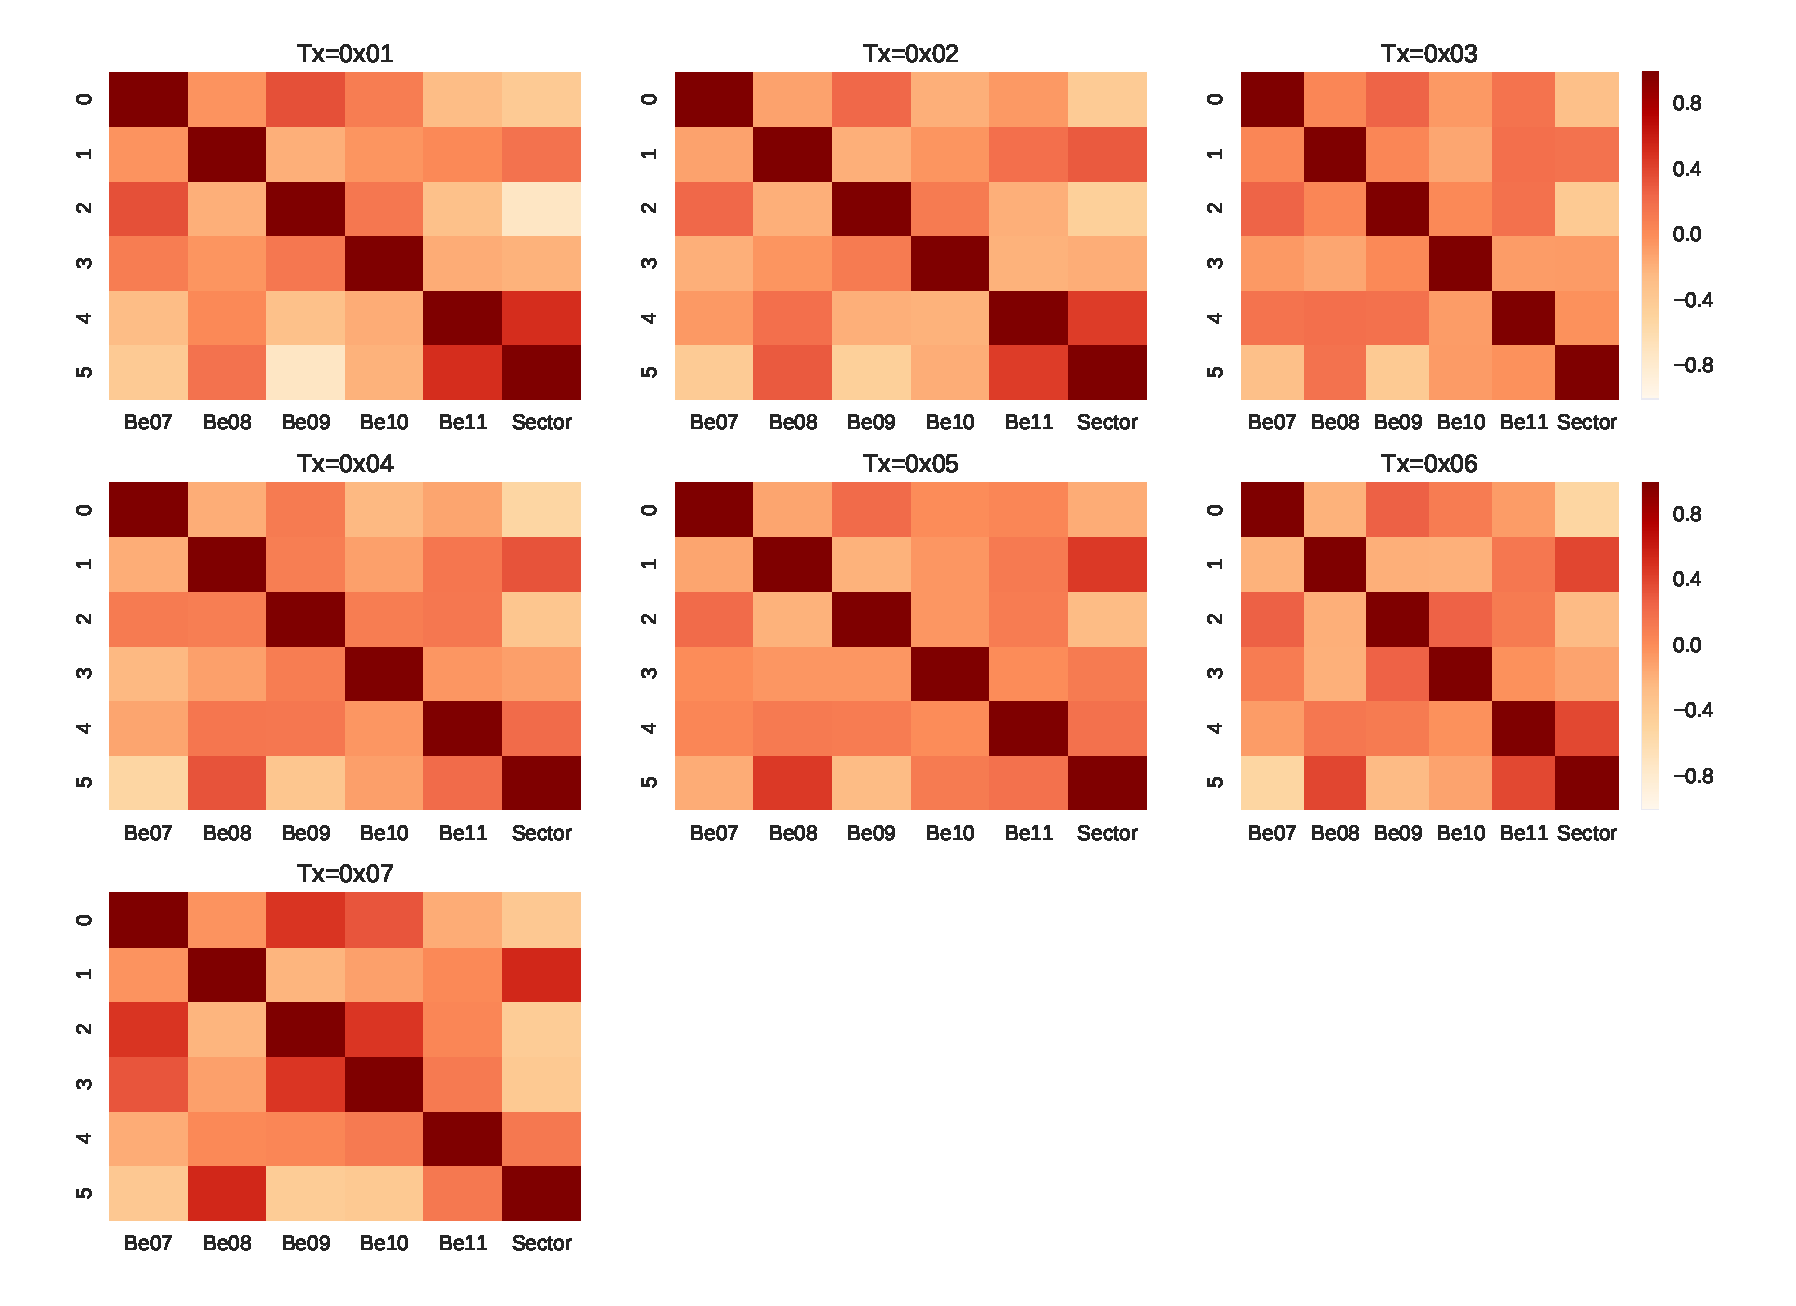
\includegraphics[scale=0.3]{AAUgraphics/correlationRaspberry.eps}
\end{center}
\end{block}
\end{frame}

\begin{frame}{Indoor Location}{Casos de Prueba}
\begin{block}{Caso 3: Beacon $\rightarrow$ Smartphone}
%Se tiene las coeficientes de correlación para los siete niveles de potencia de los beacons sobre Smartphone. En todos los casos se observa una fuerte dependencia lineal entre todos los beacons, excepto el sector.
\begin{center}
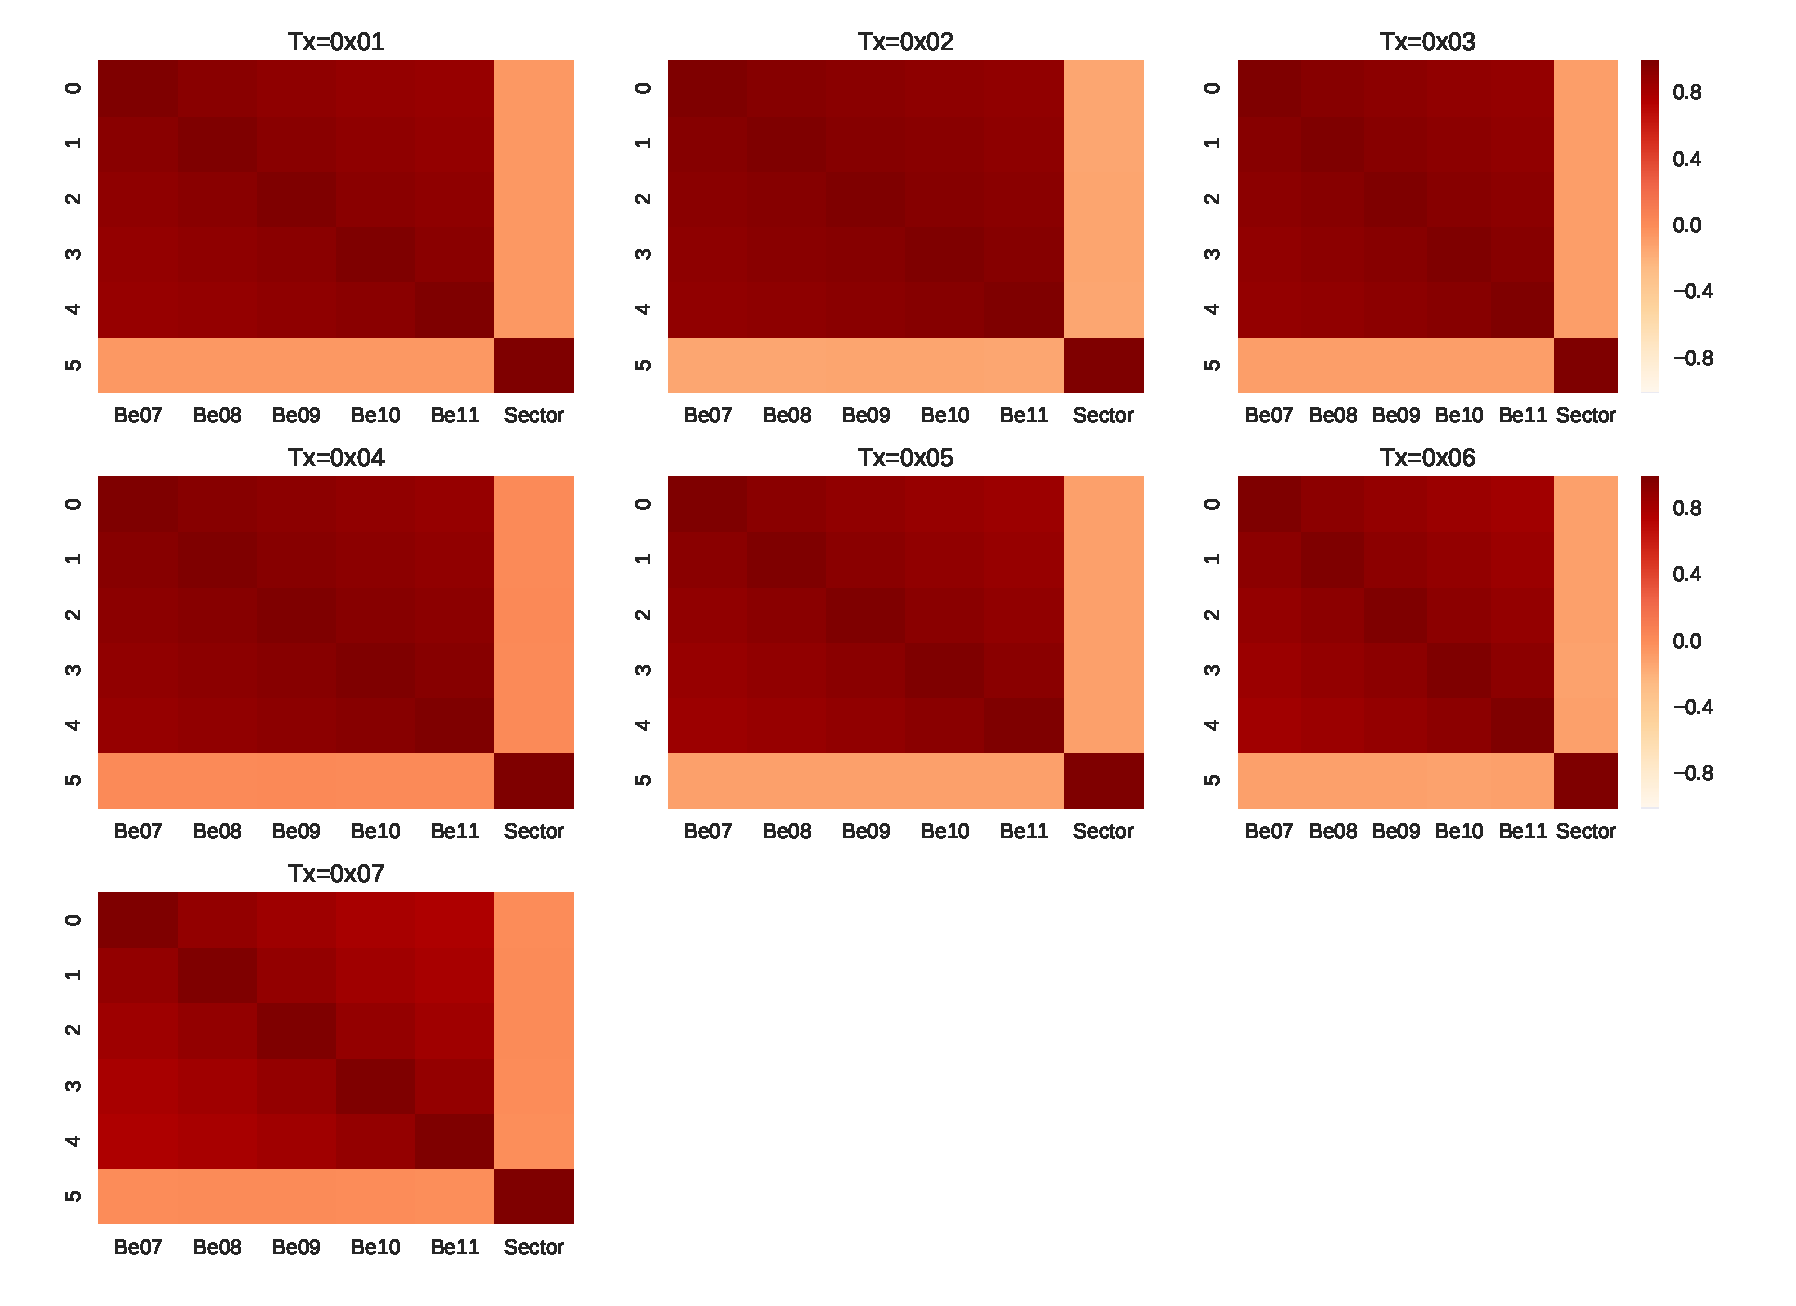
\includegraphics[scale=0.3]{AAUgraphics/correlationMoviles.eps}
\end{center}
\end{block}
\end{frame}

\subsection{Modelos de Aprendizaje}
\begin{frame}{Indoor Location}{Modelos de Aprendizaje}
%\begin{block}{Aprendizaje de M}
%https://www.quora.com/Machine-learning-is-a-broad-discipline-Where-can-I-find-a-mind-map-knowledge-tree-of-all-the-areas-and-methods-and-their-relations
%Los algoritmos de Machine Learning se dividen en dos grandes grupos, algoritmos de aprendizaje supervisado y no supervisado. Para indoor location conviene Supervised Learning.
%\begin{multicols}{2}
\begin{center}
\includegraphics[scale=0.6]{AAUgraphics/map}
\end{center}
%\\La data de entrada corresponde a vectores de cinco RSSI, y la salida el número de sector (1,2,...,15).\\
%Para modelos de clasificación los labeles de salida corresponden a [1,15]. Mientras para regresión se tomará valores reales en el mismo rango.

%Para el cálculo del error en metros se mide la distancia entre el sector real y el predicho.
%\end{multicols}
\end{frame}

\subsection{Accuracy y Error Medio}
\begin{frame}{Indoor Location}{Precisión y Error}
\begin{block}{Precisión}
%Para clasificación la precisión es el $nAciertos/nTest$, mientras que para regresión se consideran rangos, es decir $6.25<p<7.25$, entonces $p = 7$ y finalmente $nAciertos/nTest$.
$$Precision = nAciertos/nTest\times 100\%$$
\end{block}
\begin{block}{Error Métrico}
\begin{wrapfigure}{l}{0.3\textwidth}
    \centering
    \includegraphics[width=0.3\textwidth]{AAUgraphics/espacio}
\end{wrapfigure}
%El cálculo del error se realiza en metros.\\
%Para clasificación, si $p=5$ y $y=7$, el\\ error métrico corresponde a la distancia\\ entre los extremos.\\
%Para regresión, $p$ es una aproximación y\\ se toma del mismo modo.\\ Para ambos casos tenemos:
$$dv = \mid p/3 - y/3\mid\times 1.5-1.0$$
$$dh= \mid p\%3 - y\%3\mid\times 1.5-1.0$$
$$d = \sqrt{dv^2 + dh^2}$$
\end{block}
\end{frame}

\section{Resultados}
%.---------------------
% Clasificación caso 1
%.---------------------
\subsection{Caso 1}
\begin{frame}{Resultados}{Caso 1: microController $\rightarrow$ RPI2}
\begin{block}{Evaluación de Clasificación}
%Se evalua el comportamiento de los algoritmos en 10 splits con score accuracy como coeficiente de determinación sobre input data.
\includegraphics[width=1.0\textwidth]{AAUgraphics/mClass}
\end{block}
\end{frame}
%.---------------------
% Regresión caso 1
%.---------------------
\begin{frame}{Resultados}{Caso 1: microController $\rightarrow$ RPI2}
\begin{block}{Evaluación de Regresión}
%Se evalua el comportamiento de los algoritmos en 10 splits con score r2 como coeficiente de determinación sobre input data.
\includegraphics[width=1.0\textwidth]{AAUgraphics/mReg}
\end{block}
\end{frame}
%.---------------------
% tablas caso 1
%.---------------------
\begin{frame}{Resultados}{Caso 1: microController $\rightarrow$ RPI2}
\begin{multicols}{2}
\begin{block}{Clasificación}
%Resultados de precisión y\\ error métrico con data de test.\\\ \\
\includegraphics[width=0.5\textwidth]{AAUgraphics/microClasificacion}
\end{block}
\begin{block}{Regresión}
%Resultados de precisión y\\ error métrico con data de test.\\\ \\
\includegraphics[width=0.5\textwidth]{AAUgraphics/microRegresion}
\end{block}
\end{multicols}
\end{frame}
%.---------------------
% Clasificación caso 2
%.---------------------
\subsection{Caso 2}
\begin{frame}{Resultados}{Caso 2: Beacon $\rightarrow$ RPI2}
\begin{block}{Evaluación de Clasificación}
%Se evalua el comportamiento de los algoritmos en 10 splits con score accuracy como coeficiente de determinación sobre input data para $Tx=0x07$.
\includegraphics[width=1.0\textwidth]{AAUgraphics/rasTx07Class}
\end{block}
\end{frame}

\begin{frame}{Resultados}{Caso 2: Beacon $\rightarrow$ RPI2}
\begin{block}{Resultados de Precisión y Error por Clasificación}
%Resultados de precisión y error métrico obtenido por los algoritmos de clasificación para la data de test a los siete niveles de potencia.
\includegraphics[width=0.5\textwidth]{AAUgraphics/raspClasificacion}
\includegraphics[width=0.5\textwidth]{AAUgraphics/raspClasificacionErr}
\end{block}
\end{frame}
%.---------------------
% Regresión caso 2
%.---------------------
\begin{frame}{Resultados}{Caso 2: Beacon $\rightarrow$ RPI2}
\begin{block}{Evaluación de Regresión}
%Se evalua el comportamiento de los algoritmos en 10 splits con score r2 como coeficiente de determinación sobre input data para $Tx=0x07$.
\includegraphics[width=1.0\textwidth]{AAUgraphics/rasTx07Reg}
\end{block}
\end{frame}

\begin{frame}{Resultados}{Caso 2: Beacon $\rightarrow$ RPI2}
\begin{block}{Resultados de Precisión y Error por Regresión}
%Resultados de precisión y error métrico obtenido por los algoritmos de regresión para la data de test a los siete niveles de potencia.
\includegraphics[width=0.5\textwidth]{AAUgraphics/raspRegresion}
\includegraphics[width=0.5\textwidth]{AAUgraphics/raspRegresionErr}
\end{block}
\end{frame}
%.---------------------
% Clasificación caso 3
%.---------------------
\subsection{Caso 3}
\begin{frame}{Resultados}{Caso 3: Beacon $\rightarrow$ Smartphone}
\begin{block}{Evaluación de Clasificación}
%Se evalua el comportamiento de los algoritmos en 10 splits con score accuracy como coeficiente de determinación sobre input data para $Tx=0x07$.
\includegraphics[width=1.0\textwidth]{AAUgraphics/movTx07Class}
\end{block}
\end{frame}

\begin{frame}{Resultados}{Caso 3: Beacon $\rightarrow$ Smartphone}
\begin{block}{Resultados de Precisión y Error por Clasificación}
%Resultados de precisión y error métrico obtenido por los algoritmos de clasificación para la data de test a los siete niveles de potencia.
\includegraphics[width=0.5\textwidth]{AAUgraphics/movClasificacion}
\includegraphics[width=0.5\textwidth]{AAUgraphics/movClasificacionErr}
\end{block}
\end{frame}
%.---------------------
% Regresión caso 3
%.---------------------
\begin{frame}{Resultados}{Caso 3: Beacon $\rightarrow$ Smartphone}
\begin{block}{Evaluación de Regresión}
%Se evalua el comportamiento de los algoritmos en 10 splits con score r2 como coeficiente de determinación sobre input data para $Tx=0x07$.
\includegraphics[width=1.0\textwidth]{AAUgraphics/movTx07Reg}
\end{block}
\end{frame}

\begin{frame}{Resultados}{Caso 3: Beacon $\rightarrow$ Smartphone}
\begin{block}{Resultados de Precisión y Error por Regresión}
%Resultados de precisión y error métrico obtenido por los algoritmos de regresión para la data de test a los siete niveles de potencia.
\includegraphics[width=0.5\textwidth]{AAUgraphics/movRegresion}
\includegraphics[width=0.5\textwidth]{AAUgraphics/movRegresionErr}
\end{block}
\end{frame}

\section{Conclusiones}
\begin{frame}{Conclusiones}{}
\begin{itemize}
	\item A menor nivel de potencia, mayor precisión.
	\item El caso 3 presenta muy bajo
rendimiento, debido a que los cinco sensores colocados son linealmente
dependientes.
	\item El caso 2 tiene la más alta precisión, llegando hasta un
93.97\%,  muy recomendable para ambientes reducidos y de mayor afinamiento.
	\item Los algoritmos lineales en clasificación tienen menor precisión.
	\item Los algoritmos de conjunto tienen mayor precisión.
	\item Los algoritmos de clasificación tienen mayor representatividad.
	\item El error métrico promedio varía desde 0.06m hasta 1.5m a partir del extremo del sector.  
\end{itemize}
\end{frame}
%
%
%
{\aauwavesbg%
\begin{frame}[plain,noframenumbering]%
  \finalpage{Gracias por su atención}
\end{frame}}
%%%%%%%%%%%%%%%%

\end{document}
\grid
